\section{Introduction}

The problem of the project is predicting house prices in the given dataset. Since our expected values are continuously numeric values, it is a \textbf{regression} problem.\newline

We possess two datasets, namely "train" and "test," consisting of 81 columns and 2919 rows in total. These columns contain diverse information regarding basements, bedrooms, house areas, pools, garages, and more. However, both datasets suffer from numerous missing values, which need to be filled or dropped.
\newpage
\section{Data Exploration and Cleaning}
\subsection{Libraries}
\begin{enumerate}[]
  \item \textbf{Pandas}: for data frame manipulations and operations
  \item \textbf{Matplotlib}: for data visulation operations
\item \textbf{Seaboorn}: for data visulation
\item \textbf{NumPy}: for numerical operations
\item \textbf{Graphviz}: for graph  visulation 
\item \textbf{Sklearn}: for  machine learning algorithms
\item \textbf{Tensorflow}: for  deep learning



  
\end{enumerate}

\subsection{Removing Outliers}
Two datasets are given by Kaggle, train and test datasets. After reading these datasets, firstly I removed outliers on train data by looking to box plots(Figure 1). Then I combined these two datasets to make the preprocessing the same for both datasets.


\subsubsection{LotFrontage column}This column has 227 missing values. to fill these rows, I looked at the correlation between LotFrontage columns and others. As shown in the Figure 2, LotArea columns were highly correlated with LotFrontage so I used the LotArea column to fit the LotFrontage column.  After that 2 rows remain missing I filled that rows by looking 1stFlrSF column because this column was the second in the correlation table.
\begin{figure}[H]
  \centering
  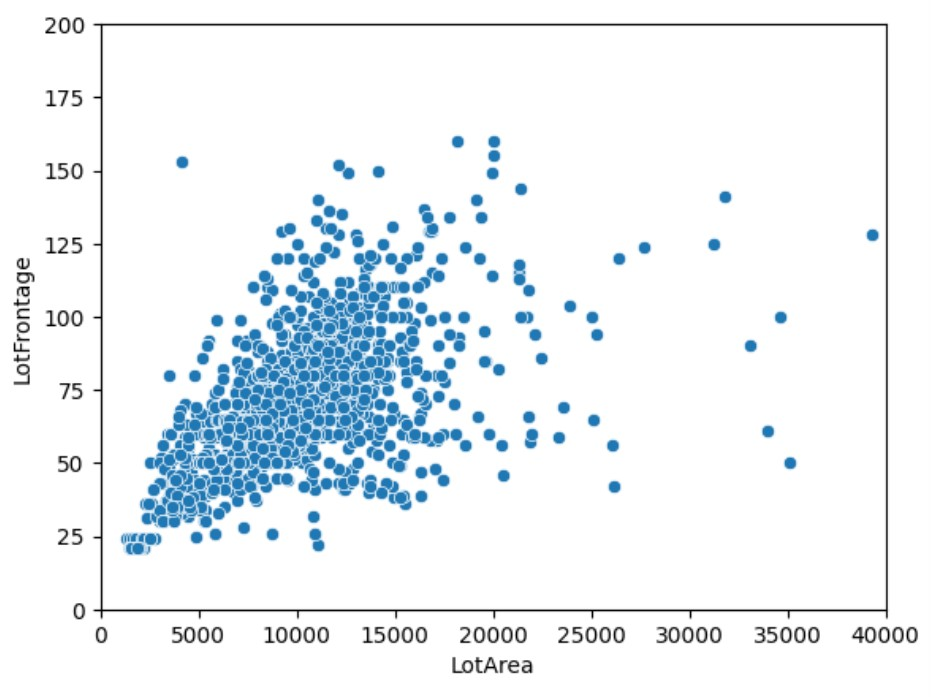
\includegraphics[width=0.5\textwidth]{./fig/lotfront.jpg}
  \label{fig:comp}
  \caption{}
\end{figure}




\subsubsection{Object columns}
MSZoning, Exterior1st, Exterior2nd, MasVnrType, Electrical, KitchenQual, Functional, and SaleType columns are filled by mode of the column since these columns have missing values less than 100.

I dropped Utilities column because it has the same values for all rows.

When I examine Basement columns I see that missing values are in the same rows. Thus, these houses have not got a Basement. I filled by "NA".

According to the description text, I filled missing values of Alley, FireplaceQu, PoolQC, Fence, and MiscFeature by "NA".




\subsection{Feature Engineering}
This dataset has been collected in 2016 so I used 2016 year to find Age of some things. I created HomeAge column by substracting 2016 from YearBuilt column. 
I created HomeAge\_ReModel column by substracting 2016 from YearRemodAdd column. 
I created GarageAge column by substracting 2016 from GarageYrBlt column. 
I created YrSold column by substracting 2016 from YrSold column. Briefly, I normalized Year columns by substracting 2016 from values.

I extracted number of Bathrooms from given features and created a new columns that is n\_bathrooms.

I created a new column that includes total area with basement.

\subsection{Replacing and changing}

After conducting thorough research on the description text, I discovered that certain columns contain values such as 'Ex,' 'Gd,' 'TA,' 'Fa,' and 'Po.' These values are used to indicate varying levels of quality or condition. Specifically, 'Ex' denotes 'Excellent,' 'Gd' represents 'Good,' 'TA' corresponds to 'Typical/Average,' 'Fa' signifies 'Fair,' and 'Po' indicates 'Poor.' However, it is important to note that these values possess a specific order, and thus, employing a label encoder to assign numerical values may result in misleading interpretations. Consequently, I decided to replace these values with alternative representations.
\begin{table}[!ht]
    \centering
    \begin{tabular}{|l|l|l|}
    \hline
        Value & Meaning & New value \\ \hline
        Ex & Excellent & 5 \\ \hline
        Gd & Good & 4 \\ \hline
        TA & Typical/Average & 3 \\ \hline
        Fa & Fair & 2 \\ \hline
        Po & Poor & 1 \\ \hline
        NA & Feature does not exist & 0 \\ \hline
    \end{tabular}
\end{table}
\newpage
\section{Predicting }
\subsection{Predicting Techniques}
First, I standardized the numerical values to ensure their comparability. However, when it came to handling the categorical variables, I faced a dilemma: whether to use dummy variables or label encoder. To make an informed decision, I decided to evaluate both approaches by training and testing 10 different models.

After conducting the evaluations, it became evident that the dataframe with dummy variables consistently outperformed the one with label encoder in 8 out of the 10 models. Therefore, I proceeded with the dataframe that employed dummy variables for further analysis and modeling. After this section, I will call df\_dum to dataframe that was created by using dummy variable.  

After realizing that there were still a large number of columns, I decided to employ various techniques to reduce the number of features.
\begin{enumerate}[]
  \item \textbf{PCA}: Principle component analysis
  \item \textbf{Correlation}: Dropping columns by looking to correlation between target column
\item \textbf{Feature Selection}: Automated feature Selection methods
\end{enumerate}
\subsubsection{PCA}

To strike a balance between reducing the number of columns and retaining sufficient information, I opted to reduce the column count from 237 to 170. By doing so, I aimed to minimize data loss while still achieving a significant reduction in dimensionality. The cumulative variance ratio obtained after the reduction was found to be 0.981, indicating that approximately 98.1\% of the original information was retained. Although a small portion of information (0.2 \%) was sacrificed, this trade-off was deemed acceptable given the substantial reduction in the number of columns. By using this PCA method on df\_dum, I created a new dataframe which is called df\_pca. Figure 2 shows the cumulative variance ratio according to the number of components.

\begin{figure}[H]
  \centering
  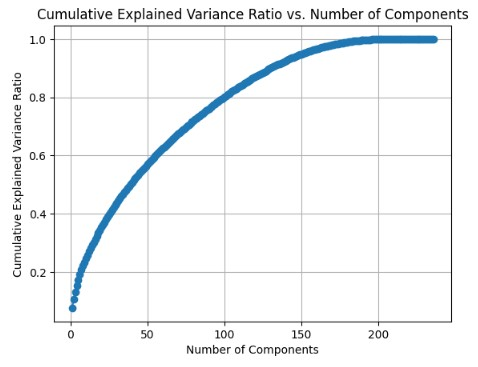
\includegraphics[width=0.5\textwidth]{./fig/cumulative.jpg}
  \label{fig:corr1}
  \caption{}
\end{figure}
\subsubsection{Correlation}

I have performed a data analysis and removed columns that exhibited a correlation coefficient of less than 0.05 with the 'SalePrice' column. This step was taken to focus on the most relevant features in relation to the target variable. By using this method on df\_dum, I created a new dataframe which is called df\_corr. Due to the large number of remaining columns (158 in total), including a heatmap table in the report would not be practical as it could be overwhelming and difficult to interpret. Therefore, the heatmap table was omitted from the report to ensure clarity and readability.


\subsubsection{Feature Selecetion}
I utilized the ExtraTreesRegressor algorithm to perform feature selection, a technique that involves evaluating the importance of each feature. By employing this method, I was able to identify and subsequently remove columns that had lower feature importance scores. This approach allows for the prioritization and retention of the most relevant features in the dataset, ultimately enhancing the efficiency and effectiveness of the analysis. By using this method on df\_dum, I created a new dataframe which is called df\_fs.

\newpage
 \subsection{Model Preparing}


During the data preprocessing, I created five different dataframes: df\_le, df\_dum, df\_pca, df\_corr, and df\_fs. To optimize the performance of each algorithm, I employed RandomizedSearchCV for hyperparameter tuning.\newline

I explored a range of machine learning algorithms, including Linear Regression, Ridge, Lasso, ElasticNet, Support Vector Machines (SVM), Decision Trees, Random Forests, GradientBoostingRegressor, ExtraTreesRegressor, KNeighborsRegressor, and VotingRegressor. Additionally, I incorporated Deep Learning techniques into my analysis. \newline

By systematically evaluating these diverse algorithms using the various dataframes, I aimed to identify the most suitable approach for my predictive modeling task. Through this iterative process, I refined the models to achieve the best possible performance.
\newpage
\section{Results}
I present the results based on the five datasets I have.
\subsection{Linear Regression}
\begin{table}[H]
\begin{tabular}{l|l|l|l|l|l|}
\cline{2-6}
                                    & \textbf{df\_le} & \textbf{df\_dum} & \textbf{df\_pca} & \textbf{df\_corr} & \textbf{df\_fs} \\ \hline
\multicolumn{1}{|l|}{\textbf{Score}} & 0.36376         & 0.1612           & 0.20618          & 0.16704           & 0.37851         \\ \hline
\end{tabular}
\end{table}


\subsection{Ridge}
\begin{table}[H]
\begin{tabular}{l|l|l|l|l|l|}
\cline{2-6}
                                   & \textbf{df\_le} & \textbf{df\_dum} & \textbf{df\_pca} & \textbf{df\_corr} & \textbf{df\_fs} \\ \hline
\multicolumn{1}{|l|}{\textbf{Score}} & 0.16462         & 0.14894           & 0.14888          & 0.14741           & 0.38088         \\ \hline
\end{tabular}
\end{table}



\subsection{Lasso}
\begin{table}[H]
\begin{tabular}{l|l|l|l|l|l|}
\cline{2-6}
                                    & \textbf{df\_le} & \textbf{df\_dum} & \textbf{df\_pca} & \textbf{df\_corr} & \textbf{df\_fs} \\ \hline
\multicolumn{1}{|l|}{\textbf{Score}} & 0.16562         & 0.14977           & 0.1582          & 0.15161           & 0.38362         \\ \hline
\end{tabular}
\end{table}


\subsection{ElasticNet}
\begin{table}[H]
\begin{tabular}{l|l|l|l|l|l|}
\cline{2-6}
                                    & \textbf{df\_le} & \textbf{df\_dum} & \textbf{df\_pca} & \textbf{df\_corr} & \textbf{df\_fs} \\ \hline
\multicolumn{1}{|l|}{\textbf{Score}} & 0.16522         & 0.14949           & 0.15711          & 0.14764           & 0.39064         \\ \hline
\end{tabular}
\end{table}







\subsection{SVR}
\begin{table}[H]
\begin{tabular}{l|l|l|l|l|l|}
\cline{2-6}
                                    & \textbf{df\_le} & \textbf{df\_dum} & \textbf{df\_pca} & \textbf{df\_corr} & \textbf{df\_fs} \\ \hline
\multicolumn{1}{|l|}{\textbf{Score}} & 0.16365         & 0.144           & 0.1525          & 0.1525           & 0.45598         \\ \hline
\end{tabular}
\end{table}








\newpage

\subsection{DecisionTreeRegressor}
\begin{table}[H]
\begin{tabular}{l|l|l|l|l|l|}
\cline{2-6}
                                    & \textbf{df\_le} & \textbf{df\_dum} & \textbf{df\_pca} & \textbf{df\_corr} & \textbf{df\_fs} \\ \hline
\multicolumn{1}{|l|}{\textbf{Score}} & 0.2314         & 0.2306           & 0.38951          & 0.25757           & 0.27437         \\ \hline
\end{tabular}
\end{table}


\begin{figure}[H]
  \centering
  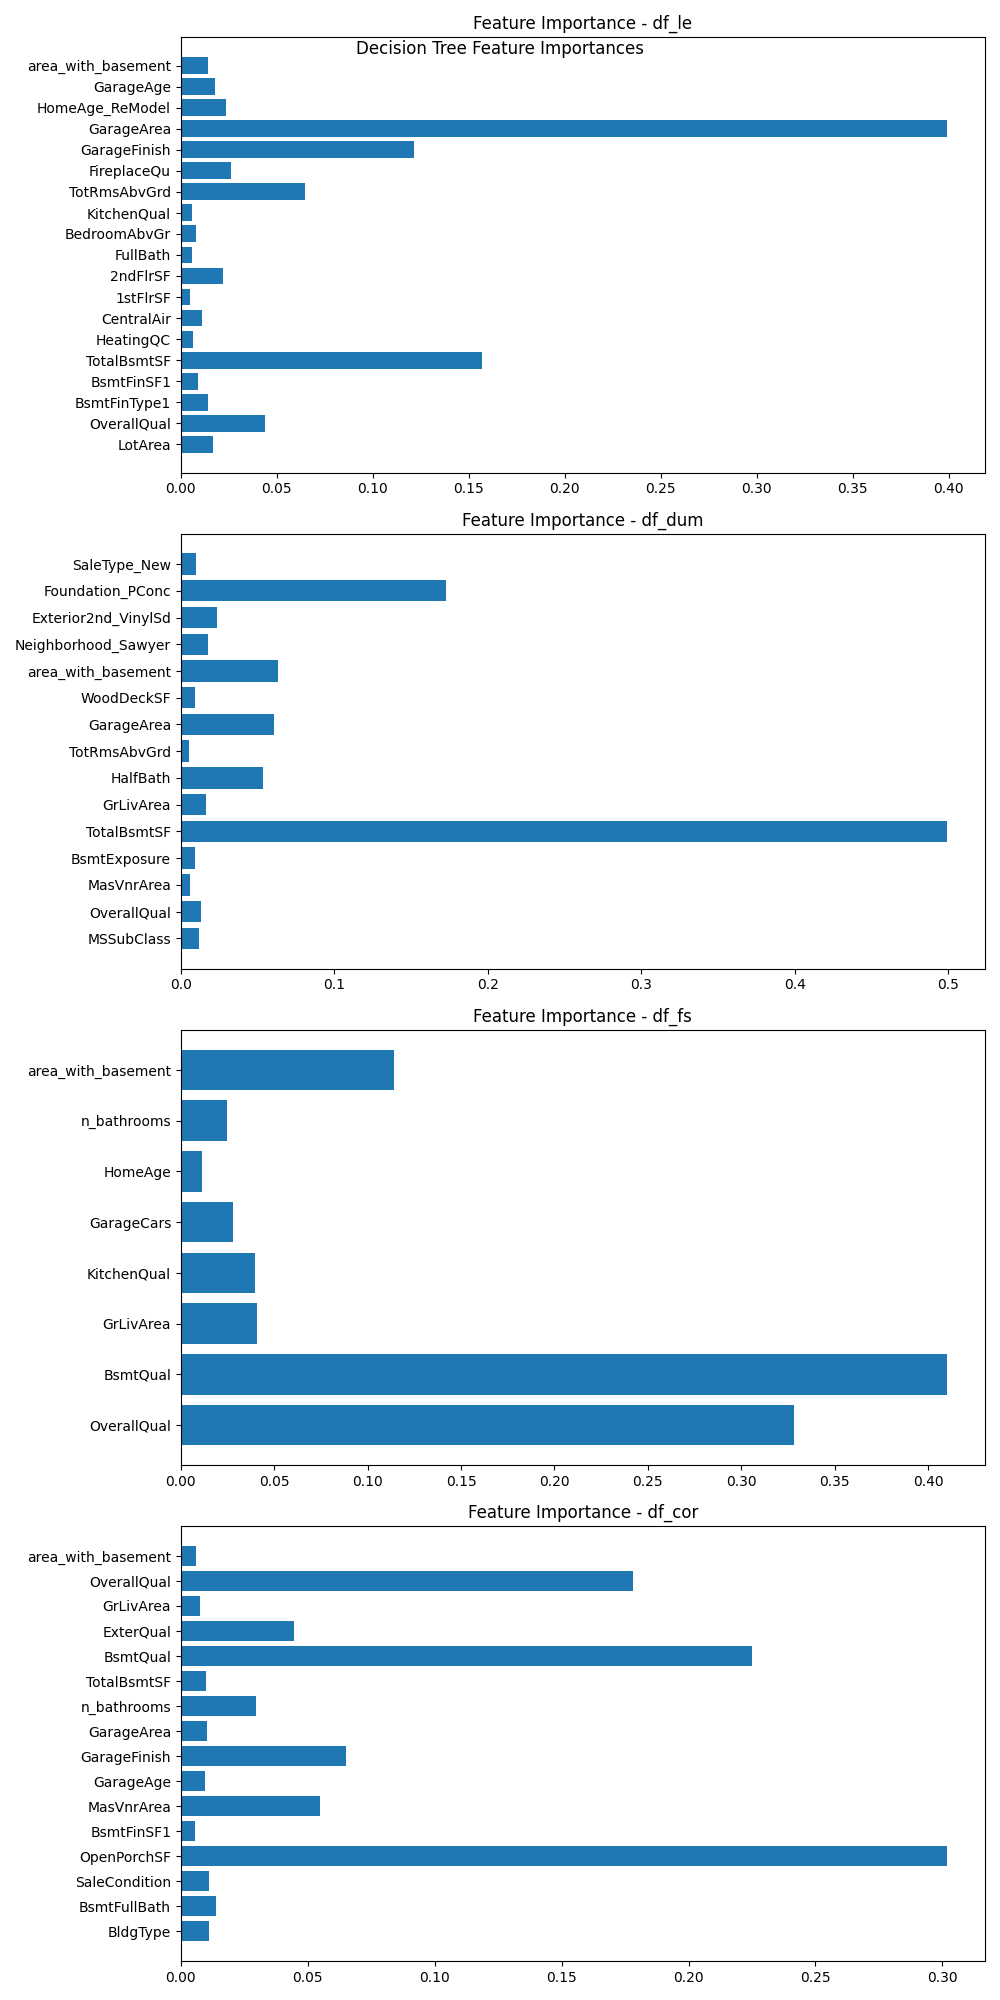
\includegraphics[width=0.53\textwidth]{./fig/featrees.png}
  \label{fig:corr1}
  \caption{}
\end{figure}








\subsection{RandomForestRegressor}
\begin{table}[H]
\begin{tabular}{l|l|l|l|l|l|}
\cline{2-6}
                                    & \textbf{df\_le} & \textbf{df\_dum} & \textbf{df\_pca} & \textbf{df\_corr} & \textbf{df\_fs} \\ \hline
\multicolumn{1}{|l|}{\textbf{Score}} & 0.16923         & 0.19343           & 0.29795          & 0.18005           & 0.25367         \\ \hline
\end{tabular}
\end{table}



\begin{figure}[H]
  \centering
  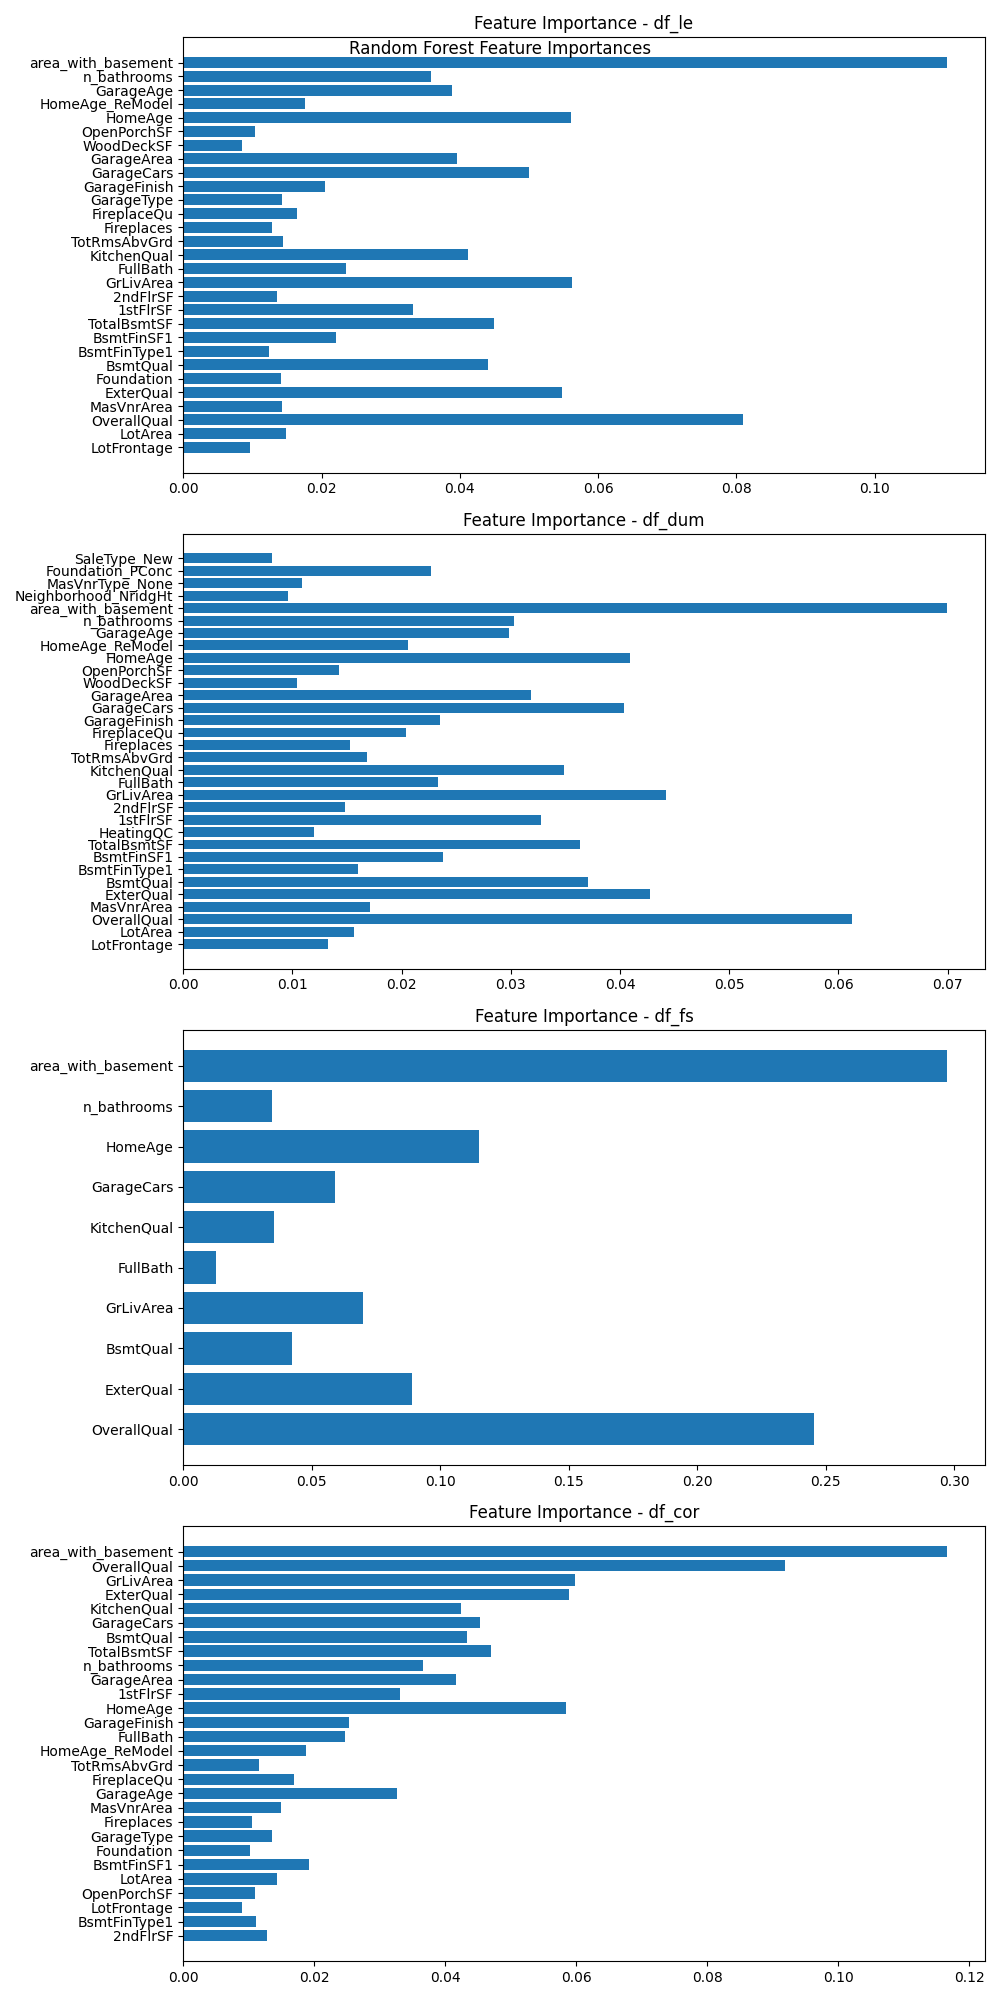
\includegraphics[width=0.53\textwidth]{./fig/ranfeas.png}
  \label{fig:corr1}
  \caption{}
\end{figure}









\subsection{ExtreTreesRegressor}
\begin{table}[H]
\begin{tabular}{l|l|l|l|l|l|}
\cline{2-6}
                                    & \textbf{df\_le} & \textbf{df\_dum} & \textbf{df\_pca} & \textbf{df\_corr} & \textbf{df\_fs} \\ \hline
\multicolumn{1}{|l|}{\textbf{Score}} & 0.24288         & 0.27196           & 0.38737          & 0.24906           & 0.31774         \\ \hline
\end{tabular}
\end{table}



\begin{figure}[H]
  \centering
  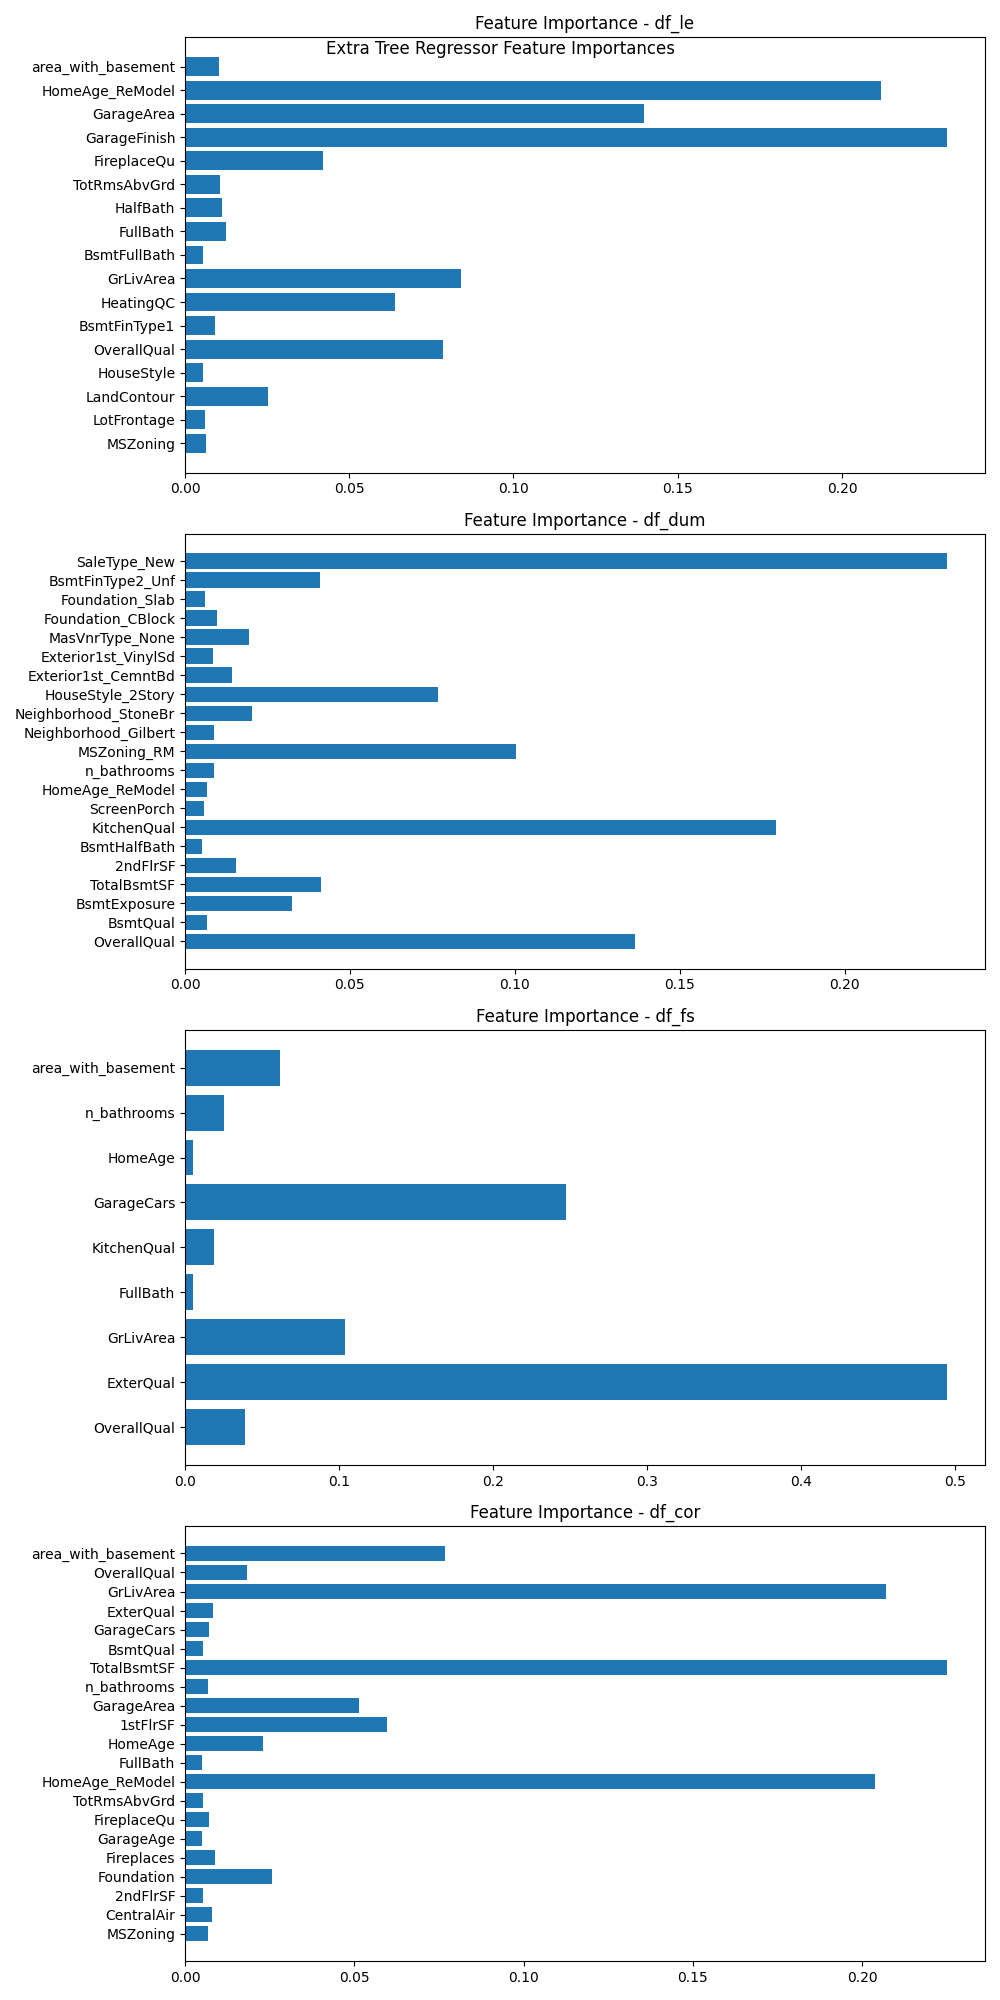
\includegraphics[width=0.53\textwidth]{./fig/etcfeas.png}
  \label{fig:corr1}
  \caption{}
\end{figure}








\subsection{GradientBoostingRegressor}
\begin{table}[H]
\begin{tabular}{l|l|l|l|l|l|}
\cline{2-6}
                                    & \textbf{df\_le} & \textbf{df\_dum} & \textbf{df\_pca} & \textbf{df\_corr} & \textbf{df\_fs} \\ \hline
\multicolumn{1}{|l|}{\textbf{Score}} & 0.13769         & 0.1361           & 0.23008          & 0.14098           & 0.31107         \\ \hline
\end{tabular}
\end{table}



\begin{figure}[H]
  \centering
  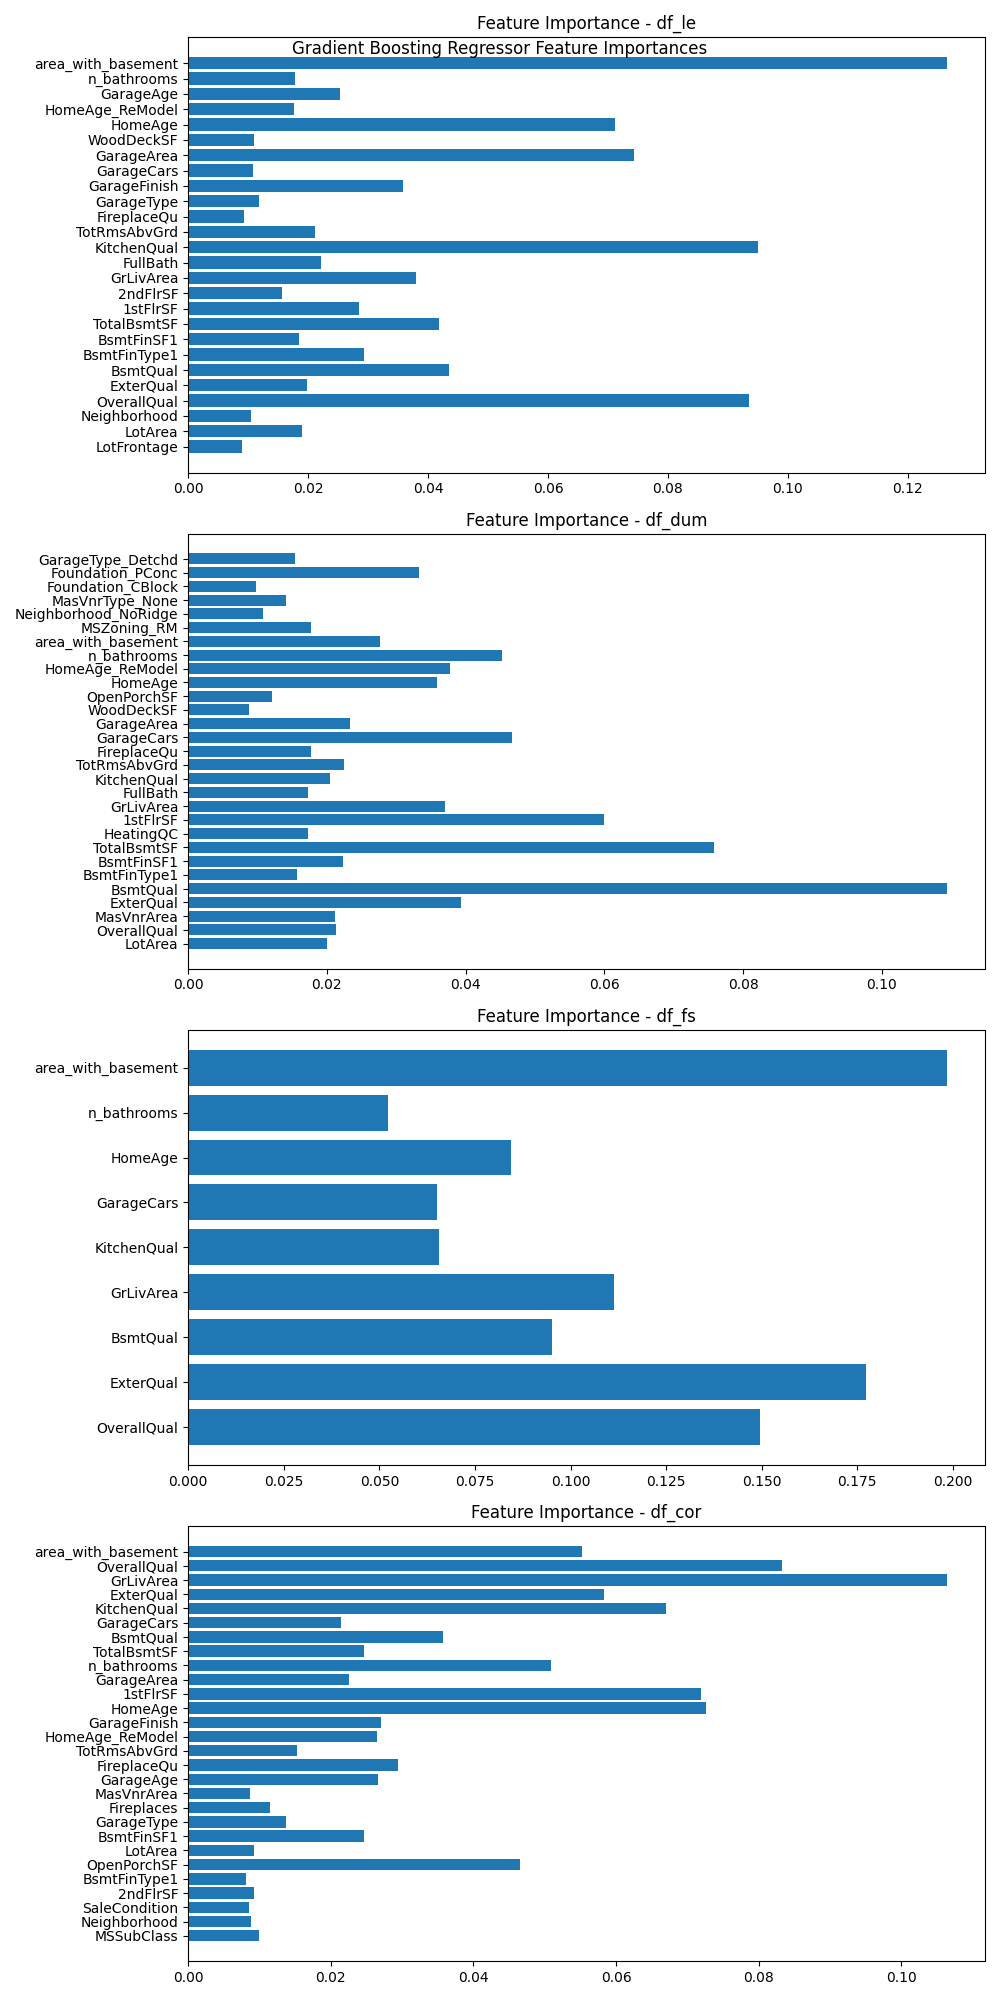
\includegraphics[width=0.53\textwidth]{./fig/GradientBoostingRegressor.png}
  \label{fig:corr1}
  \caption{}
\end{figure}








\subsection{KNN}
\begin{table}[H]
\begin{tabular}{l|l|l|l|l|l|}
\cline{2-6}
                                   & \textbf{df\_le} & \textbf{df\_dum} & \textbf{df\_pca} & \textbf{df\_corr} & \textbf{df\_fs} \\ \hline
\multicolumn{1}{|l|}{\textbf{Score}} & 0.19372         & 0.18937           & 0.19511          & 0.16968           & 0.20701         \\ \hline
\end{tabular}
\end{table}


\subsection{Deep Learning}

In my deep learning experiments, I initially employed four different models to tackle the task at hand. The first model solely consisted of dense layers, while the second model incorporated l1 regularization. For the third model, I introduced dropout layers to enhance generalization, and in the fourth model, I implemented batch normalization to improve the stability of the training process.

However, upon evaluating the performance of these models, I observed that the accuracy of the last two models significantly decreased compared to the initial dense model. To manage my limited submission rights or constraints, I decided to remove the third and fourth models from consideration. 

Since I do not have test data I did not use validation and test in deep learning.
\begin{enumerate}[]
  \item \textbf{Model that includes only Dense layers}: 
  \begin{table}[H]
\begin{tabular}{l|l|l|l|l|l|}
\cline{2-6}
                                   & \textbf{df\_le} & \textbf{df\_dum} & \textbf{df\_pca} & \textbf{df\_corr} & \textbf{df\_fs} \\ \hline
\multicolumn{1}{|l|}{\textbf{Score}} & 0.14399         & 0.14951           & 0.18914          & 0.14176           & 0.15536         \\ \hline
\end{tabular}
\end{table}



\begin{figure}[H]
  \centering
  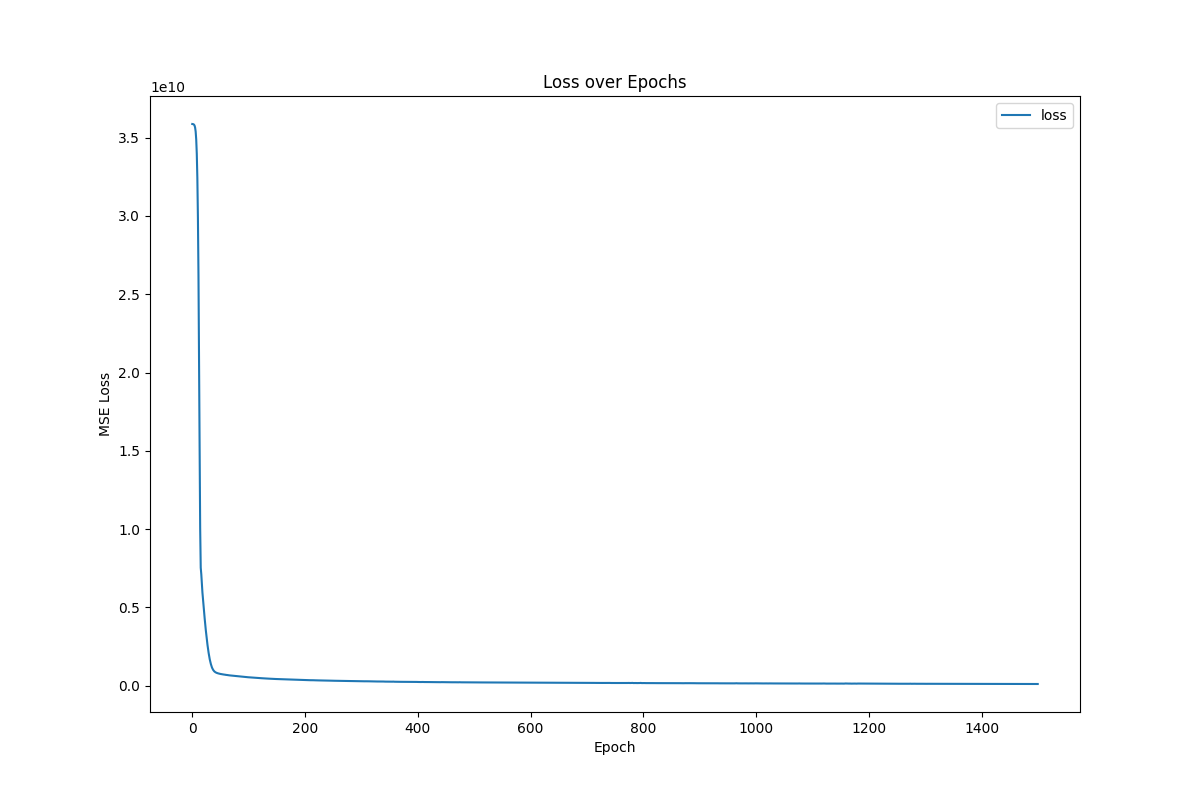
\includegraphics[width=0.7\textwidth]{./fig/losofdeep.png}
  \label{fig:corr1}
  \caption{Loss over epoch for this model}
\end{figure}




  \item \textbf{Model with L1 Regularization}: 
\begin{table}[H]
\begin{tabular}{l|l|l|l|l|l|}
\cline{2-6}
                                   & \textbf{df\_le} & \textbf{df\_dum} & \textbf{df\_pca} & \textbf{df\_corr} & \textbf{df\_fs} \\ \hline
\multicolumn{1}{|l|}{\textbf{Score}} & 0.14233         & 0.15258           & 0.18515          & 0.14375           & 0.16472         \\ \hline
\end{tabular}
\end{table}
  
\begin{figure}[H]
  \centering
  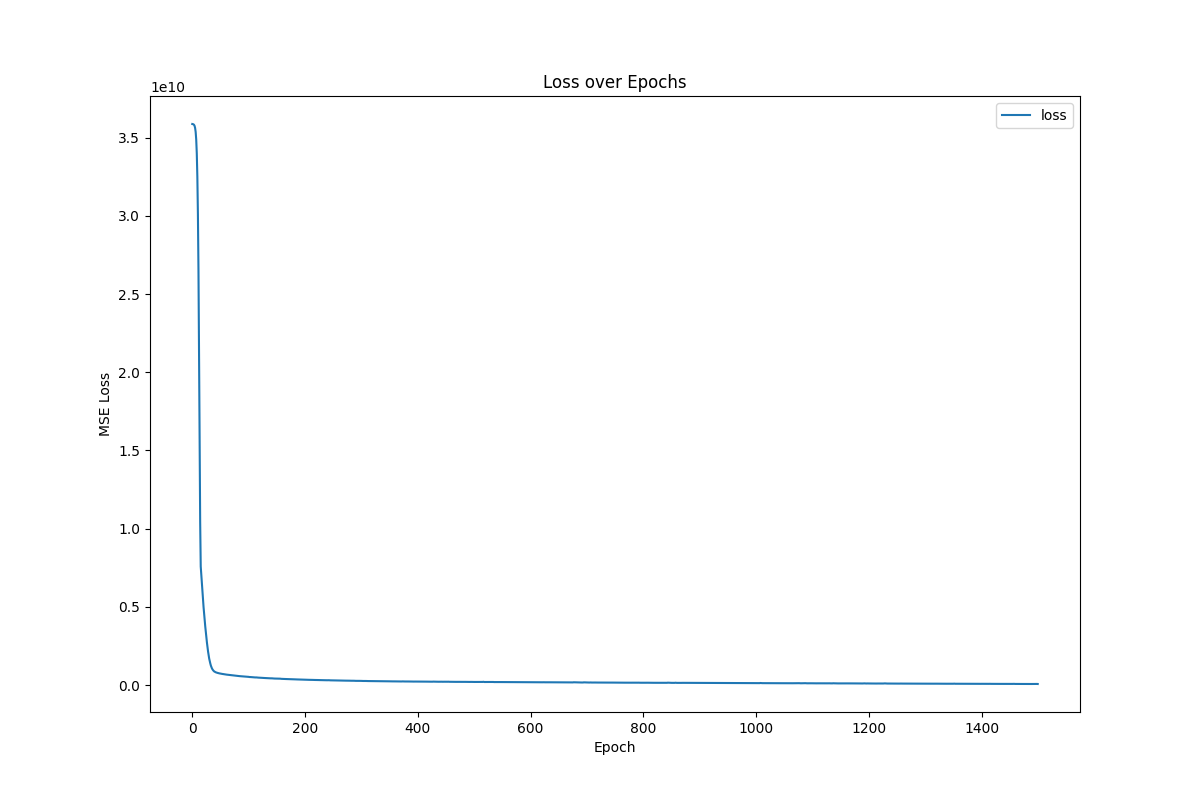
\includegraphics[width=0.7\textwidth]{./fig/losofregdeeep.png}
  \label{fig:corr1}
  \caption{Loss over epoch for this model}
\end{figure}
\end{enumerate}
When I look at the loss function it seems like the model overfitted however when I decrease the epoch number accuracy decreased to so I fixed 1500 epoch number.

To better results, we need more data, in small sizes data machine learning models give better results than deep learning. 

\newpage
\subsection{VotingRegressor}
 In Voting Regressor, I used three approaches. Firstly, I used all models. Secondly, I used the best 7 models.Finally, I used models that have more than 0.20 accuracy. In the Voting Regressor I didnt use df\_fs because it gives worst accuracy in models so I decied to not use it in Voting regressor.\newline
\begin{enumerate}[]
  \item \textbf{With all models}: 
\begin{table}[H]
\begin{tabular}{l|l|l|l|l|}
\cline{2-5}
                                     & \textbf{df\_le} & \textbf{df\_dum} & \textbf{df\_pca} & \textbf{df\_corr} \\ \hline
\multicolumn{1}{|l|}{\textbf{Score}} & 0.14261         & 0.14           & 0.17195          & 0.14113           \\ \hline
\end{tabular}
\end{table}



  \item \textbf{Best 7 models}: 
\begin{table}[H]
\begin{tabular}{l|l|l|l|l|}
\cline{2-5}
                                     & \textbf{df\_le} & \textbf{df\_dum} & \textbf{df\_pca} & \textbf{df\_corr} \\ \hline
\multicolumn{1}{|l|}{\textbf{Score}} & 0.13604         & 0.13191           & 0.13969          & 0.13309           \\ \hline
\end{tabular}
\end{table}
  \item \textbf{Models have more than 0.20 accuracy}: 

\begin{table}[H]
\begin{tabular}{l|l|l|l|l|}
\cline{2-5}
                                     & \textbf{df\_le} & \textbf{df\_dum} & \textbf{df\_pca} & \textbf{df\_corr} \\ \hline
\multicolumn{1}{|l|}{\textbf{Score}} & 0.138         & 0.1367           & 0.15098          & 0.13569           \\ \hline
\end{tabular}
\end{table}
\end{enumerate}
\section{Best Score}
My Best score is 0.13191.


\begin{figure}[H]
  \centering
  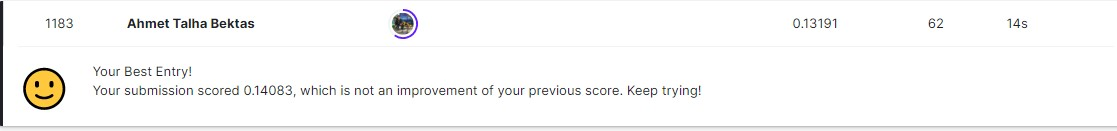
\includegraphics[width=1\textwidth]{./fig/best.jpg}
  \label{fig:corr1}
  \caption{}
\end{figure}
\newpage
\begin{thebibliography}{6}

	\bibitem{blog1} 
	Brownlee, J. (2020, March 30). How to Calculate Feature Importance With Python. Retrieved from https://machinelearningmastery.com/calculate-feature-importance-with-python/
 
	\bibitem{blog2} 
	Anuganti, S. (2020, November 30). How to Remove Outliers for Machine Learning? Analytics Vidhya. Retrieved from https://medium.com/analytics-vidhya/how-to-remove-outliers-for-machine-learning-24620c4657e8


	\bibitem{blog3}
		Tan, E. (2022, February 7). How to Fill Missing Data with Pandas. Towards Data Science. https://towardsdatascience.com/how-to-fill-missing-data-with-pandas-8cb875362a0d
\bibitem{blog4}
		Yalçın Er, B. (2020, October 18). Label Encoding ve One Hot Encoding. Retrieved from https://mertmekatronik.com/label-encoding-ve-one-hot-encoding  	


\bibitem{blog5}
		Singh, A. (2018, June 18). A Comprehensive Guide to Ensemble Learning. Analytics Vidhya. Retrieved from https://www.analyticsvidhya.com/blog/2018/06/comprehensive-guide-for-ensemble-models/
\end{thebibliography}